\chapter{Proposed incremental changes for a conventional tide service to compliment modern applications}

%----------------------------------------------------------
% content variables
%----------------------------------------------------------
% define variables for antt station ids used in figure names
\newcommand{\Ba}{63540}
\newcommand{\Ca}{46290}
\newcommand{\Da}{62430}
\newcommand{\Ea}{62290}
\newcommand{\Fa}{61561}
\newcommand{\Ga}{57720}

\newcommand{\Bb}{529020}
\newcommand{\Cb}{200970}
\newcommand{\Db}{005096}
\newcommand{\Eb}{008314}
\newcommand{\Fb}{523757}
\newcommand{\Gb}{200854}

\newcommand{\Bname}{Mornington Island}
\newcommand{\Cname}{Christmas Island}
\newcommand{\Dname}{Point Murat}
\newcommand{\Ename}{Geraldton}
\newcommand{\Fname}{Cape Jervis}
\newcommand{\Gname}{Lord Howe Island}

\newcommand{\figwidthFull}{0.75\textwidth}
\newcommand{\figwidthHalf}{0.35\textwidth}
\newcommand{\figwidthThird}{0.22\textwidth}
%------------------------------------------------
% main
%------------------------------------------------
\section{Introduction}
\label{Sec:intro}
%--------------------------
This paper asserts that conventional tide prediction services will better compliment modern forecasting by adopting appropriate data categories for machine-to-machine delivery.   Emphasis is placed on clarifying easily confused tidal concepts and demonstrating differences with operational data.   
Section \ref{Sec:intro} characterises the place of conventional tidal prediction within an operational agency with diverse uses beyond navigation. Section \ref{Sec:OfficialGlobal} highlights the different representational aims of standard tides and physical tide models with respect to the underlying physics.   Section \ref{Sec:DoubleCount} addresses the implications of including meteorologically dominated tides and doubling counting signals when hybridising with other water level data. Section \ref{Sec:Evolution} explores an operational archive of Australian tidal analysis to demonstrate that constants and offsets evolve with the traditional annual tides update.   Finally Section \ref{Sec:proposed} proposes a minimal set of data ``flavours'' that could help ensure an automated machine-to-machine tide service best compliments the modern requirements. 


\subsection{Modern data micro-services and earth system modelling}
National forecasting agencies are increasingly providing machine-readable online data to support the diverse downstream economy of value-adding and combination.
This `micro-service' architecture \citep{BCG2020} is increasingly relevant to government services and is embodied by programs such as  \url{https://api.gov.au/}) and the International Hydrographic Organisations  navigation-focused exchange specifications (\url{http://s100.iho.int}).

 
Earth system modelling and forecasting continues to increase in sophistication along the dimensions of representational 'concreteness' \citep{Petersen:2012kp}, forecast duration, assimilation of observations and combination into seamless services \cite{BOM2020}.
Within this context, coastal sea level is the subject of a diverse range of productive development activity very often centred on high resolution and down-scaled numerical simulations \citep{10.3389/fmars.2019.00437}. 


Despite all the advances in earth system modelling, conventional tide prediction is a unique and persistent form of forecast that is well-suited to on-demand delivery.  Tide predictions are an input to many systems, have relatively tiny data volumes and are built on a conceptual foundation that allows for cheap synthesis of timeseries at arbitrary times.    There are several global examples of on-demand machine-readable tidal data service such as  \url{https://tidesandcurrents.noaa.gov/tide_predictions.html}, but nothing yet from an Australian agency and none that are known to distinguish variants for different applications.


Automated delivery raises the attractive potential to synthesise tidal timeseries at any arbitrary times required by a user; whether in the past or the future.   But without critical assessment,  there is a risk that such a service may unfortunately imply that tidal sea levels are an uncomplicated and singular thing.    
Whilst this simple view may be no problem for many applications, the following discussion highlights why tidal data would be better treated like other analysis and forecast services by clearly distinguishing some variants or data ``flavours''. 
Appropriate distinction of tidal data types would clarify the compatibility of the content whilst allowing developers and users to remain relatively isolated from backend details and processing improvements on the part of the supplier.

%--------------------------
\subsection{Why conventional tide predictions are still relevant}

Terminology surrounding ocean tides rarely helps with clarity of communication.  But it is hard to ignore that daily variations in sea level are dominated by overtly tidal signals in most coastal locations.  Godin colourfully remarked that when inspecting spectra of observed sea level variability from tide gauges ``the constituent lines emerge from the noise background as trees from the gras'' \cite{godin:1972}.
The ability to fit and exploit time-invariant admittance relationships between the patterns of astronomical motions and observed sea level records is an early and great success of mathematical geophysics \cite{Cartwright:2000tt} that derives unique ``\textit{forecasting power.. from the infinite extent of its basis functions} ''\citep{Flinchem:2000kp}.

Conventional tidal sea level products are well embedded into coastal economies.   The ability to span very long forecast horizons to accurately predict the timing of phenomena on a sub-hourly timescale is unique. 
The products are however so well embedded and useful as to be somewhat taken for granted and sometimes treated uncritically. 


\subsection{National agency practice and diverse uses}

In Australia, harmonic tidal analysis and prediction has been routinely carried out by government agencies for several decades.  For navigation purposes the Australian Hydrographic Service promulgates an annual official set of port predictions in the form of the Australian National Tide Tables (ANTT) and its software version AusTides.   AusTides is not an automated data delivery service, but rather stand alone electronic version of the tide tables.  
The majority of the analysis behind the tide tables is carried out by the Bureau of Meteorology at the the National Tide Centre.  
The analyses are founded on a harmonic least-squares method implemented within a proprietary suite of software that traces a lineage to the Proudman institute \citep{MHL2156}.    
The Bureau and various other state agencies publish annual tide predictions at locations additional to the ANTT. 
This well established practice of routine tidal analysis and prediction can be called ``conventional''.


The downstream application of these tidal sea-level products is not limited to navigation.   
In fact, the range of contemporary uses motivates the present discussion; for instance:
\begin{inparaenum}[1)]
    \item land survey and cadastral references - mean sea level and tidal planes such as ``highest astronomical tide'' 
    \item hydrographic survey, charted depths and clearances
    \item long term planning for coastal works and installations
    \item short term forecasts for coastal activities 
    \item filtering (de-tiding) of sea level observations
    \item input into data-driven decision support systems
    \item combination with physical forecasts into seamless water level forecasts 
    \item verification and tuning of hydrodynamic modeling
\end{inparaenum}

A notable aspect of national tide services is the special status of promulgating predictions that are considered ``official''.   For some applications it could be argued this status is more important than forecast accuracy alone.
  
  

Conventional tidal analysis has some unique and attractive features from an operational maintenance perspective.
At face value, the practice is robust to data-stream outages in that poor quality and historical observations can still be exploited to produce predictions.  
Annual batch-mode production schedules are far less demanding than real-time continual forecast systems. 
The harmonic method compresses results to a few dozen  human-readable parameters that are amenable to routine quality checking and error detection. 
Conventional tidal analysis at port locations can be characterised as a slow-motion data-driven method that is somewhat physics-free; especially when compared to modern hydrodynamic simulations. 

Figure \ref{fig:tidePractice} portrays the unique way that conventional tidal practice can transform heterogeneous historical records into a consistent timeseries product at arbitrary time sampling.
The pragmatic role of experts in managing what is now commonly  called ``data wrangling'' and merging non-uniform and auxiliary sources is a notable contrast to fully automated systems.
 
\begin{figure}[H]\centering
        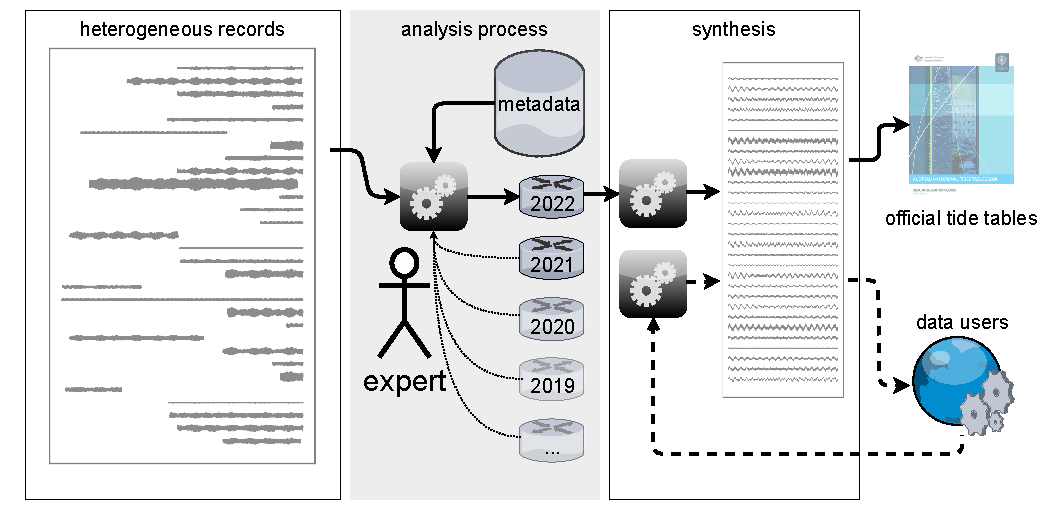
\includegraphics[width=\figwidthFull]{figures/diagrams/tideSchematic.pdf} 
        \caption{Schematic to illustrate how a conventional tidal process manages heterogeneous data sources on an annual update cycle.  Official tide requirements are not identical to those of all data users. }
        \label{fig:tidePractice}
\end{figure}   


Growing access to real-time quality observations both remote and insitu has to potential to tip the balance of value away from conventional tidal and even physical simulations at shorter timescales (eg \citep{10.3389/fmars.2019.00437}, \citep{10.3389/fmars.2020.00260} ), but perhaps not so much across the longer scales of months to years that conventional products are relied upon.
Furthermore the pragmatic matters of applying quality flags, managing supplier inhomogeneity and relatively sparse spatial coverage remain non-trivial problems in Australia.


But despite the fact that the unique properties of conventional tide products seem to guarantee some ongoing relevance, there is a need to ensure that these products are designed and delivered in a manner that is fit-for-purpose without inviting needless representational error. 


%--------------------------
\subsection{Precedent for data differentiation in remote observations and other forecasts}

Most simply, the distinction between a forecast and an ``analysis'' would not be possible if an automated tidal service provided a single all-purpose synthesised signal.
This distinction is obvious to users of weather forecast data and other oceanographic products (eg \url{https://marine.copernicus.eu/}) but arguably tidal predictions have to date maintained an exceptional product status; tides a thought of as more akin to the manifestation of a Platonic form than just another \textit{model} output \citep{Jay:2003bj} \citep{10.1029/2018rg000636}.


The operational delivery of remote  observations of sea level has well established distinctions between what could be called data `flavours'.   Both with regard to the distinction between rapid update interim products and behind-real-time quality analysis as well as the wide range of geophysical  correction combinations that are suited to different applications ( eg \citep{Scharroo:2014vv} )


Allowing for the effective operational use of standard tide products in the context of satellite observations raises the significance of basic compatibility 
issues such as vertical reference datums \citep{10.3389/fmars.2020.549467}.
Similarly, whilst remote observations of sea level anomalies (SLA) are a critical constraint on operational non-tidal forecasts \citep{10.1080/1755876x.2019.1685834}, any extension to render tide gauge data into the same format would require compatible tidal corrections - and corrections differ in intent from offical port predictions.


%------------------------------------------------
\section{Problem: tide models and standard predictions don't have a shared aim}
\label{Sec:OfficialGlobal}

One underlying motivation for distinguishing official from physical tide data is the role of dynamic ocean simulations in the operational environment.  
Global tide solutions are a foundational oceanographic product that in rough approximation extends the tradition of tidal analysis well away from tide gauges.   Similar to conventional tidal techniques, these solutions conceptualise the ocean as a linear-time-invariant (LTI) system forced by the tidal gravity patterns associated with the relative motion of the earth, moon and sun.   The surface height predictions from global tide solutions allow for the decomposition of remote ocean observations into tidal and nontidal components, but are also widely used for other extension applications.
In contrast to the advancing ability of physical ocean circulation forecasts to explicitly include tides (eg \cite{10.1016/j.ocemod.2019.02.008}), global LTI tide solutions share the unique ability of conventional prediction methods to efficiently provide data at the arbitrary times required by the application.

For instance, the national inter-tidal extent mapping exercise of \cite{10.3390/rs10030480}  directly applied global model predictions in part for the machine-readable and on-demand availability.
Various Australian studies of water level \ref{Haigh:2013bn}\ref{Pattiaratchi2018} and more recently currents \cite{10.5194/os-2020-107} all apply timeseries synthesised from global model solutions to provide model boundary conditions at what ever time period is required.    Such down-scaling simulations are often motivated by the reasonable expectation of adding simulation value at the time and length scales afforded by higher spatial resolution.   But the longer scales bring to attention the manner in which the aims of physical models and standard predictions differ.

\subsection{Intentional differences - especially for long period tides}
Harmonic developments of the tidal potential include relatively a weak species referred to as the long period tides.  Some of the long period constituents are known by conventional names such as \textbf{Sa}, \textbf{Ssa}, \textbf{Mm},\textbf{Msf} and \textbf{Mf}; see \cite[table 4] {10.1016/b978-0-444-53802-4.00058-0}.
Conventional tidal prediction applies the essentially the same statistical fitting procedure to the long period tides as to the more familiar tidal periods of around one day and shorter; though usually with some inclusion caveats based on the observational record. 
But regardless of record length, the treatment of long period tides highlight a difference in the aims of conventional tide prediction and modern tide models.   Namely the extent to which it is desirable to fit patterns that are primarily the result of non-astronomical phenomena.
Parker's tide manual states that ``\textit{whether the calculated values of Sa and Ssa are used or not, becomes almost a philosophical question...and may not represent the annual cycle for a particular year very well anyway}''  \citep[Section 3.7]{Parker:2007wq} 

Physical approaches to the quantifying global long period tides \citep{Egbert:1994wz} do not result in amplitudes anything like those resulting for conventional tide gauge records; especially for when relatively short records and significant nontidal power noise is involved.   Amplitudes of over 20cm are used in places along the Australian coast as shown in Figure \ref{fig:SaAmp}. On the other hand, when an annual ``best'' forecast of sea level is the target it is understandable that \textit{any} pattern found to be periodic enough to project onto the tidal basis functions is included in the synthesis of the prediction. 
Even if this intentional difference is known to specialists, downstream users of an automated tidal data service are at risk of building in needless representational error if the distinction is not designed clearly into the service.


A similar situation exists for the generally tiny but weather-dominated daily constituent S1 \cite{Ray:2004ts}.


%"it is well known that [the] representation of the slow variation of the levels is inadequate" [pp216]\citep{godin:1972} 

\begin{figure}[H]\centering
    \begin{subfigure}[b]{\figwidthFull}
        \includegraphics[trim={0 0 0 1cm},clip,width=\textwidth]{figures/maps/locations_noM2Update.png} \caption{Over 650 mixed-quality stations on record based on heterogeneous inputs}
    \end{subfigure}
    \\
    \begin{subfigure}[b]{\figwidthFull}
        \includegraphics[trim={0 0 0 1cm},clip,width=\textwidth]{figures/maps/locations_anyM2UpdatePha.png} \caption{Only 132 stations with recently updated analyses. Named locations as per text.}
    \end{subfigure}
    \caption{Amplitude and phase of seasonal component \textbf{Sa} at locations with tidal analysis records}
    \label{fig:SaAmp}
\end{figure}   

In contrast to conventional tidal analysis, the widely used Oregon State University Tide Prediction Software \citep{Egbert:2002ug} [hereafter \textbf{TPXO}] totally excludes Sa, Ssa, Msf and S1; but both include Mm and Mf.  Subsequently any application that brings both type of prediction into the same context, even if indirectly, requires some caution to avoid representational inconsistency. 


\subsection{Inter-representation agreement}
Given that the amplitudes of even the conventionally determined long period tides are generally rather small and that most tidal evaluations are carried out in frequency space, the following evaluation aims to demonstrate the practical implications when handling synthesised timeseries.

Variants of 15 minute tide predictions at all Australian sites for the full year of 2020 are used for comparison.   TPXO predictions were generated using the standard interpolation to site locations and sites where excluded that fell beyond the solution grid.   The National Tide Centre in-house software (unpublished) was modified to selectively exclude particular constituents in order to generate alternative quasi-official predictions for the study period.  All prediction time series for this comparison are relative to MSL (more on that in Section \ref{Sec:MSL}).  

It is expected that a global tide solution will not represent all the localised and shallow-water patterns that a conventional analysis can capture.   However the aim of this evaluation is to highlight the arguably less-expected but intentional representational difference at primarily meteorological or `radiational' tides \cite{10.1016/b978-0-444-53802-4.00058-0}.   To this end a the following improvement metric is shown on the summary map in Figure \ref{fig:improveOtps}.
\begin{equation}
    I = 1- \frac{rms(\eta_{B}-\eta_{TPXO})}{rms(\eta_{A}-\eta_{TPXO})}
    \label{eq:improvment}
\end{equation}
With water level timeseries $\eta$ variants:
\begin{inparaenum}
[A)]
    \item port tides with all constituents; 
    \item port tides with excluded constituents individually and in combination: Sa, Ssa, Mm, Msf, Mf and S1.
\end{inparaenum}

The total removal of primarily meteorological constituents consistently improves the compatibility of the physical and conventional predictions as is expected.   Moreover, improvement in agreement is partially contributed by each individual constituent with the only case for any ambiguity being Mf. Mf is the strongest of the long period forcing terms but still overall the results indicate that the conventional tide attribution is skewed towards the projection of nontidal noise (see Figure \ref{fig:williamsFraction} panel [e] as well). 


NOTE - confim nodal modulation in OTPS


\begin{figure}[H]\centering    
    \begin{subfigure}[b]{\figwidthFull}
        \includegraphics[trim={0 0 0 1cm},clip,width=\textwidth]{figures/maps/otpsPortCompare_Improve2020_201_diffRmse.png}
        \caption{Improvement metric due to all exclusions}
    \end{subfigure}
    \\
    \begin{subfigure}[b]{\figwidthFull}
        \includegraphics[width=\textwidth]{figures/plots/compareTides_\Fa_Full2020.png} 
        \caption{\Fname{} with all constituents}
    \end{subfigure}
    \\
    \begin{subfigure}[b]{\figwidthFull}
        \includegraphics[width=\textwidth]{figures/plots/compareTides_\Fa_2020_105.png} 
        \caption{\Fname{} with exclusions}
    \end{subfigure}
    \caption{Representational agreement between global TPXO tide model and 'official' port tides is improved by total removal of weather dominated constituents from the later.   Predictions relative to MSL.  Metric is unitless - see Figure \ref{fig:SaAmp} for \textbf{Sa} amplitudes.}
    \label{fig:improveOtps}
\end{figure}   


%------------------------------------------------
\section{Problem: Double-counting risk when combining tides with forecasts}
\label{Sec:DoubleCount}
A practical implication of a lack of clarity when using tidal data services is the risk of ``double-counting'' signal; especially when hybridising tide data with physical models. 
Williams \cite{10.5194/os-2020-107} described this risk and made evaluations based on the tidal analysis of global barotropic ocean simulations for single one year period. 
The supplementary data supplied by Williams are used to visualise the power attributed to wind and pressure effects and shown in Figure \ref{fig:williamsFraction}.  The spatially consistent high ratios for long periods and S1 stands in stark contrast to the small fractions attributed to the other constituents.    
For the purposes of providing a tidal data service that can facilitate hybrid applications (eg \cite{Taylor:2017coa}) whilst mitigating double-counting, these evaluations suggest that simply excluding the long periods and S1 in total would be a reasonable starting point.   This is discussed further in  section \ref{Sec:proposed}.
This simple interpretation of the Williams evaluation intentionally underplays the details of phase and wave interaction effects to focus on the gross differences in representational aim between physical models and standard tide predictions. 
The ``\textit{possibility that ... non-tidal power is leaking into the Mm and Mf estimates}'' in this short model analysis is arguably a dominant effect for many Australian tide predictions - discussed in section \ref{Sec:Evolution}.
A barotropic ocean model evaluation of course excludes the possible projection of steric and ocean circulation phenomena on tide predictions based on observations; as is the possible role of internal-tides modulating signals in locations such as North Western Australia \citep{10.3389/fmars.2021.629372}.

It is notable that long period signals in Australian sea level studies are quite reasonably always the subject of special treatment. For instance Haigh \cite{Haigh:2013bn} and Pattiaratchi \cite{10.1074/mcp.s800908-mcp200} ensure that long period signals are appropriately filtered, fit or replaced to account for the representational limits of barotropic models when interpreting results against observations.
Arguably a tidal data service that provides prediction types excluding these  predominantly non-tidal effects could better compliment physical modelling applications along these lines. 


\begin{figure}[H]\centering
    \begin{subfigure}[b]{\figwidthHalf}
        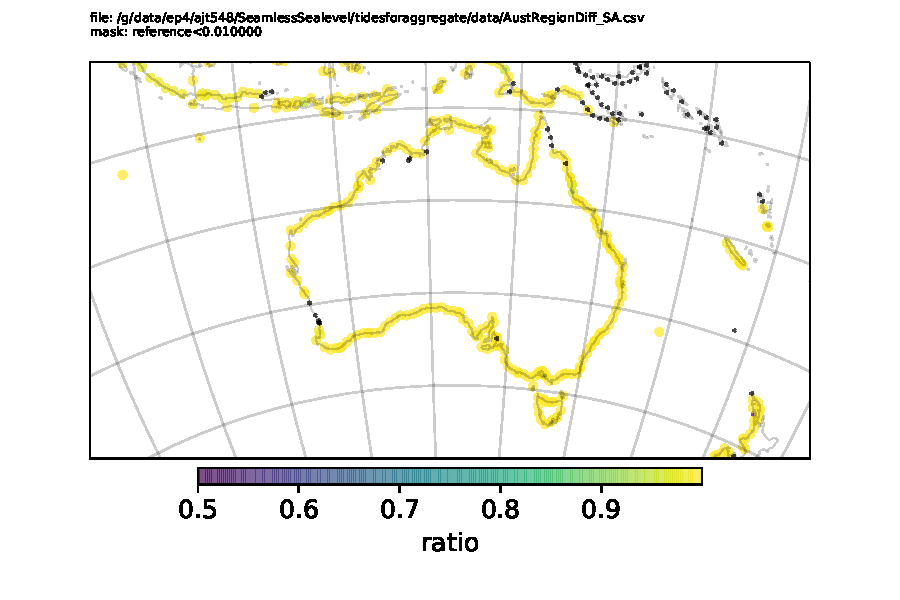
\includegraphics[width=\textwidth]{figures/maps/AustRegionDiff_SA.pdf}
        \caption{SA}
    \end{subfigure}
    \begin{subfigure}[b]{\figwidthHalf}
        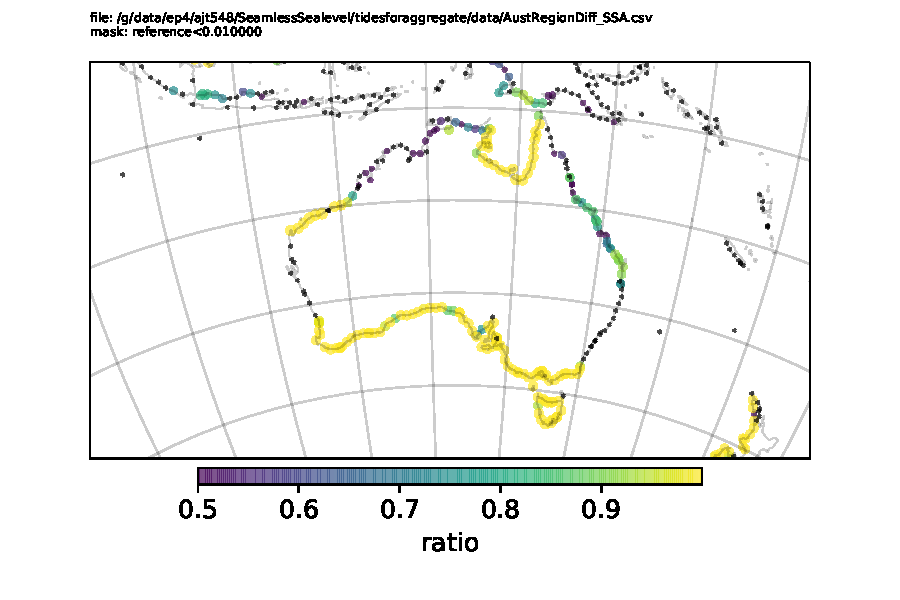
\includegraphics[width=\textwidth]{figures/maps/AustRegionDiff_SSA.pdf}
        \caption{SSA}
    \end{subfigure}
    \begin{subfigure}[b]{\figwidthHalf}
        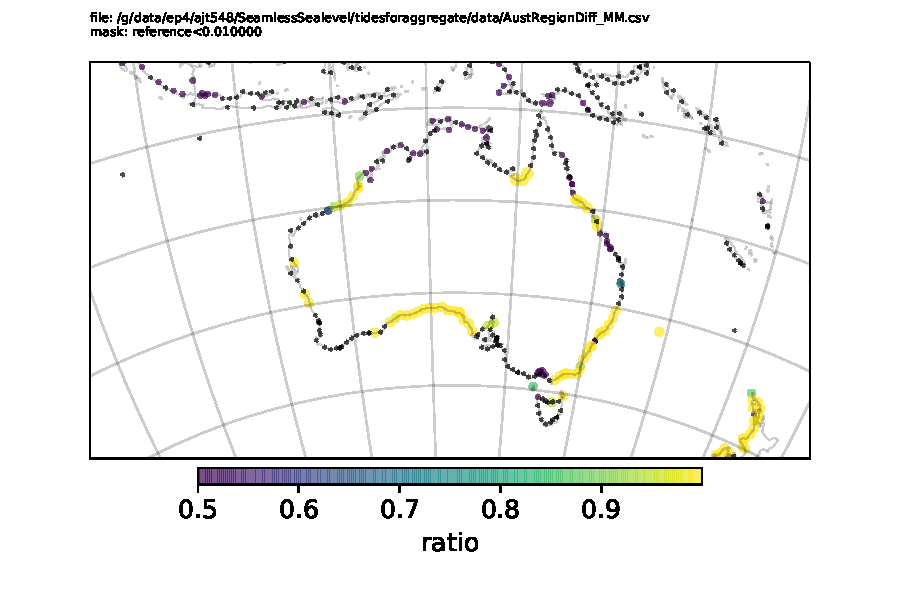
\includegraphics[width=\textwidth]{figures/maps/AustRegionDiff_MM.pdf}
        \caption{MM}
    \end{subfigure}
    \begin{subfigure}[b]{\figwidthHalf}
        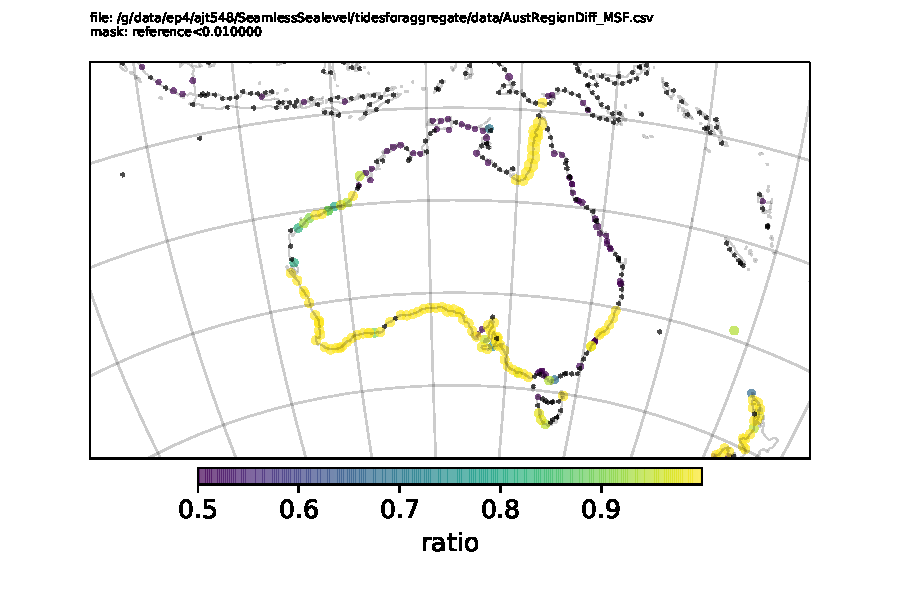
\includegraphics[width=\textwidth]{figures/maps/AustRegionDiff_MSF.pdf}
        \caption{MSF}
    \end{subfigure}
    \begin{subfigure}[b]{\figwidthHalf}
        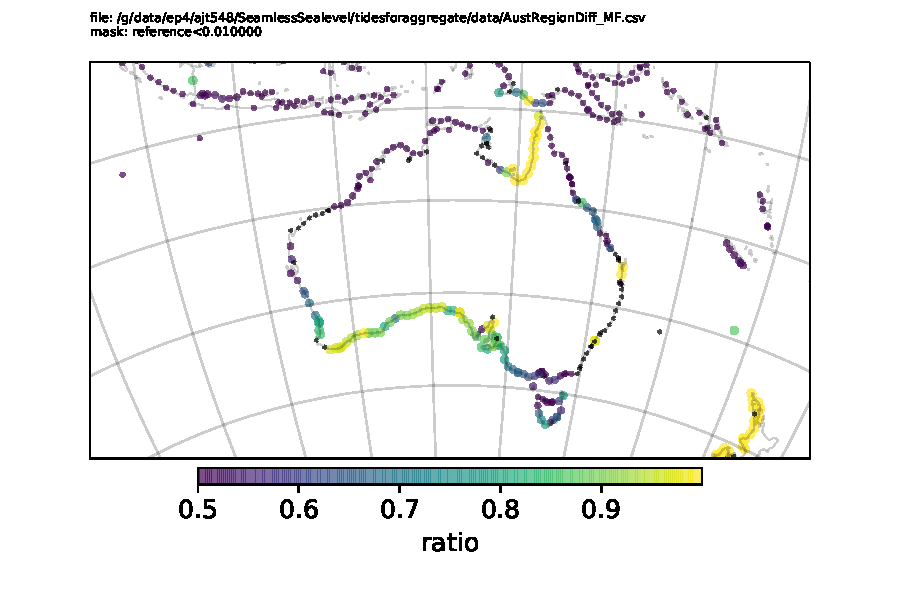
\includegraphics[width=\textwidth]{figures/maps/AustRegionDiff_MF.pdf}
        \caption{MF}
    \end{subfigure}
    \begin{subfigure}[b]{\figwidthHalf}
        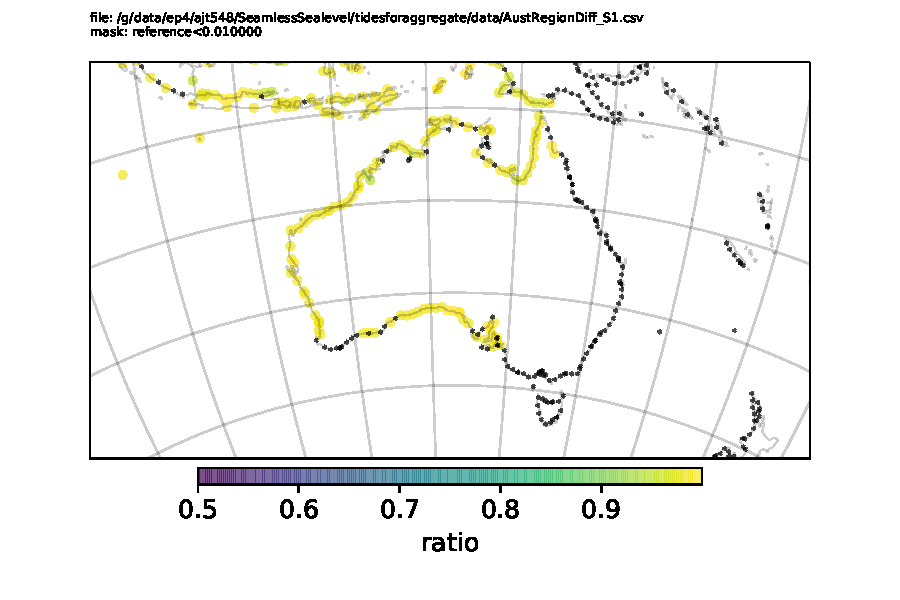
\includegraphics[width=\textwidth]{figures/maps/AustRegionDiff_S1.pdf}
        \caption{S1}
    \end{subfigure}
    \caption{Fraction of tidal amplitude attributed to wind and pressure effects from Williams\cite{10.5194/os-2020-107}.  Based only on amplitude and ignoring magnitudes $<1$cm.  As a starting estimate, the observational-based standard analysis of these constituents could be categorised as primarily non-astronomical.}
    \label{fig:williamsFraction}
\end{figure}



The practical impact of double-counting is ...at these focus stations and reason for choice.
All have recent forecasting relevance, real time observations and something challenging or unique from a conventional tidal prediction perspective.
While the ideal for tidal analysis is a very long high quality record of continuous observations, in practice this cannot be relied upon.



% insert table
\begin{table}[H]\centering
\begin{tabular}{ r|p{1cm}|p{1.2cm}|c|c|c }
Name 
 & ANTT 
 & BoM 
 & web  
 & port type
 & Obs for 2022
  \\ 
\toprule
Mornington Island 
 & 63540 
 & 529020 
 & Y 
 & Secondary 
 & 30/06/2007 - 31/12/2016
 \\
Christmas Island  
 & 46290 
 & 200970 
 & Y 
 & Secondary 
 & 04/08/2009 - 31/12/2018
 \\
Point Murat       
 & 62430 
 & 005096 
 & Y 
 & Secondary 
 & 13/05/2008 - 31/12/2019
 \\
Geraldton         
 & 62290 
 & 008314 
 & Y
 & Primary   
 & 01/01/1985 - 31/12/2019
 \\
Cape Jervis       
 & 61561 
 & 523757 
 & N 
 & Secondary
 & 29/05/2014 - 31/12/2019
 \\
Lord Howe Island  
 & 57720 
 & 200854  
 & Y 
 & Secondary 
 & 02/08/1994 - 31/12/2019
 
 \\
\end{tabular}
\label{tab:sites}
\end{table}


Statistics based on aggregate sea level with/without correct tide.


\begin{figure}[H]\centering
    % B
    \begin{subfigure}[b]{\figwidthThird}
        \includegraphics[width=\textwidth]{figures/plots/ObsError_\Bb.png}\caption{\Bname{}}
    \end{subfigure}
    % C
    \begin{subfigure}[b]{\figwidthThird}
        \includegraphics[width=\textwidth]{figures/plots/ObsError_\Cb.png}\caption{\Cname{}}
    \end{subfigure}
    % D
    \begin{subfigure}[b]{\figwidthThird}
        \includegraphics[width=\textwidth]{figures/plots/ObsError_\Db.png}\caption{\Dname{}}
    \end{subfigure}
    \\
    % E
    \begin{subfigure}[b]{\figwidthThird}
        \includegraphics[width=\textwidth]{figures/plots/ObsError_\Eb.png}\caption{\Ename{}}
    \end{subfigure}
    % F
    \begin{subfigure}[b]{\figwidthThird}
        \includegraphics[width=\textwidth]{figures/plots/ObsError_\Fb.png} \caption{\Fname{}}
    \end{subfigure}
    % G
    \begin{subfigure}[b]{\figwidthThird}
        \includegraphics[width=\textwidth]{figures/plots/ObsError_\Gb.png} \caption{\Gname{}}
    \end{subfigure}
    \caption{Forecast model sea level linearly superposed with two variants of the standard tide prediction: [A] all constituents (official) and [B] exclusion of nominally weather dominated (weather-free).  Operational data for ~ three years. Record means removed. } 
    \label{fig:tideOverlay}
\end{figure}   


%------------------------------------------------
\section{Problem: `constants' are not really constant}
\label{Sec:Evolution}
The prospect of an automated on-demand tidal service raises another motivation for clarifying data types; that of the stability of tidal parameters across time.

Australian tidal agencies do not systematically publish the parameters associated with the annual tidal production cycle; expect for the subset of constituent values at select sites that are supplied with the nautical publications \cite{austides}.    The following evaluation is believed to be the first account of the temporal evolution of parameters behind these official predictions.  

Conventional tidal parlance reflects an effective aim for the annual analysis that is to better identify a time-invariant admittance relationship characterised by a set of constants; constants that ideally wouldn't change if only we knew them well enough. Flinchem characterises this as old clockwork and  line-spectrum framework \cite{Flinchem:2000kp}. 

In contrast, Colosi and Munk assert that ``\textit{variability in the values of tidal `constants' should be the rule rather than the exception!}'' \cite{Colosi:2006va}
The expectation of temporal instability for tidal constants has recently been further elaborated by Hague \cite{10.1029/2018rg000636} and Devin \cite{10.1002/2017jc013165} amongst others.    This reasonable characterisation obviously presents some level of conceptual incompatibility with standard practice.

Inspection of annual changes across the archive of analysis parameters first and foremost highlights the wide range of sources and heterogeneous inputs managed to produce tide tables - as characterised in Figure \ref{fig:tidePractice}.    Whilst the ability to derive value from such a range is a great strength of conventional practice, the resulting predictions  should be accompanied by rankable quality measures as proposed in Section \ref{Sec:proposed}.
The evolution of tidal parameters across the archive is addressed below in two parts relevant to a prospective automated tidal data service:  updates to nominally weather-dominated harmonics and then updates to the separation of MSL from prediction datum.

Of all the sites on the archive, only a subset are based on tide gauges stations that are both in operation and supplying data to the agency for analysis. When new observations are available the annual analysis typically extends the length of record analysed.   The analysis of a continually accumulating record is consistent with the aim of better fitting a set of constants; but is in contrast to studies specifically investigating non-stationary tidal evolution such as Devin \cite{10.1002/2017jc013165}.
As an indication of how actively updated tidal parameters actually are, the full set of well over 600 tidal locations was reduced to around 130 that had any change to the 5 significant figures attributed to M2 amplitude since 2011 - this shown by the reduction in sites between panels in Figure \ref{fig:SaAmp}.


%--------------------------
\subsection{Harmonics}
The annual changes at sites details table \ref{tab:sites} and in Figure \ref{fig:complexEvolution}.
Importantly, these are mainly secondary ports in which the observational record is known to be somehow sub-optimal.    However they are all sites of operational relevance that serve to support the expectation that the weather dominated constituents are subject to projection of quasi-periodic or even aperiodic signals not a=driven by the tidal potential.  

\begin{figure}[H]\centering
    % B
    \begin{subfigure}[b]{\figwidthHalf}
        \includegraphics[width=\textwidth]{figures/plots/complex_\Ba.pdf}\caption{\Bname{}}
    \end{subfigure}
    % C
    \begin{subfigure}[b]{\figwidthHalf}
        \includegraphics[width=\textwidth]{figures/plots/complex_\Ca.pdf}\caption{\Cname{}}
    \end{subfigure} 
    \\
    % D
    \begin{subfigure}[b]{\figwidthHalf}
        \includegraphics[width=\textwidth]{figures/plots/complex_\Da.pdf}\caption{\Dname{}}
    \end{subfigure}
    % E
    \begin{subfigure}[b]{\figwidthHalf}
        \includegraphics[width=\textwidth]{figures/plots/complex_\Ea.pdf}\caption{\Ename{}}
    \end{subfigure}
    \\
    % F
    \begin{subfigure}[b]{\figwidthHalf}
        \includegraphics[width=\textwidth]{figures/plots/complex_\Fa.pdf} \caption{\Fname{}}
    \end{subfigure}
    % G
    \begin{subfigure}[b]{\figwidthHalf}
        \includegraphics[width=\textwidth]{figures/plots/complex_\Ga.pdf} \caption{\Gname{}}
    \end{subfigure}
    \caption{Evolution of annual updates to select constituents at focus sites displayed as both phasors and smaller timeseries of amplitude and phase.  Annual results are not independent due to accumulating input data. Relatively radical changes reflect the power of quasi-periodic variability at these frequencies as well as the heterogeneous record quality on which analyses are based} 
    \label{fig:complexEvolution}
\end{figure}   


Comments about the different stations ....
Power of Sa.


Relative stability of Gero ....Leuwin current check



%--------------------------
\subsection{Mean sea level}
\label{Sec:MSL}
What counts as background or mean sea level is context-dependant. 

\cite{Haigh:2013bn} considers MSL to be a time varying background sea level signal.

As does the official Australian predictions are accompanied by this explanation:
``\textit{Wherever possible, predictions are based on continuous observation of the tide over a period of at least one year, in such cases the average changes in mean sea level due to changes in meteorological conditions for the year in question are calculated and included in the predictions.  These changes do not, however, repeat themselves exactly from year to year; it has been advisable, therefore, to observe and analysis changes in mean sea level for a period of not less than three years.   In case of modern analyses, this practice has been increasingly adopted}'' \cite{austides}

Different treatments of MSL change patterns in Australia have been singled out as a source of inter-agency inconsistency with room for improvement \cite{MHL2156}.


In contrast, for survey applications MSL as a static value and its decomposition to separate the dynamic topography component has a special relevance. \cite{Filmer:2018cu}


But for ``weather-free'' tidal timeseries it would be appropriate to simple report the values relative to MSL.

\cite{10.1007/s11069-021-04600-4} in a longer-term projection context.   Doesnt account for admittance change, but intuitive guide.



The elevation of MSL relative to PD is updated annually for Australian predictions ....more than one reason.
Disctinct from the long period harmonics discussed above ...

\begin{figure}[H]\centering
    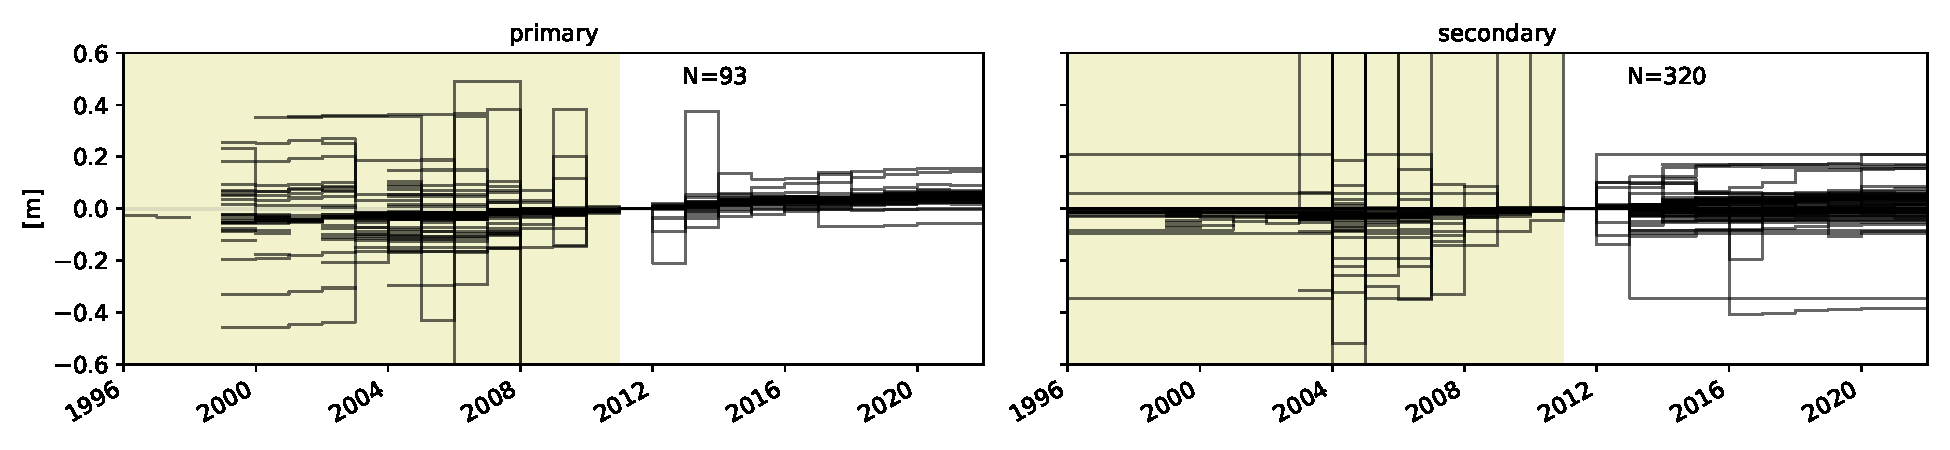
\includegraphics[width=\figwidthFull]{figures/plots/Z0_evolution.pdf}
        \caption{Evolution of zero frequency levels used for annual tide predictions at primary and secondary ports. Changes relative to arbitrary zero year of 2011. Variations reflect the heterogeneity of sources and potential for offset discontinuities with API delivery}
    \label{fig:z0Evolution}
\end{figure}   



\subsection{Timeseries data relevance}
The annual update to official parameters is undertaken with the specific goal  of improving stand-alone water level predictions for the year ahead.    It should come as no surprise that this practice may introduce discontinuities when looking back over historical predictions.
But looking back at official data is exactly what some users of an automated data service may require and it is important that there is no confusion about what data is being supplied.
Compare this to an application where the aim is simply to estimate the tidal water level variability component  for a historical period regardless of what was official or available at the time.
Figure \ref{fig:tideOverlay} illustrates the difference for the case of  \Dname{}.  The evolving long period characteristics of the official annual updates can be compared to panel [c] in Figure \ref{fig:complexEvolution} recalling that these operational values represent a growing input record and a independent observations such in the studies of Devin \cite{10.1002/2017jc013165}. 

\begin{figure}[H]\centering
    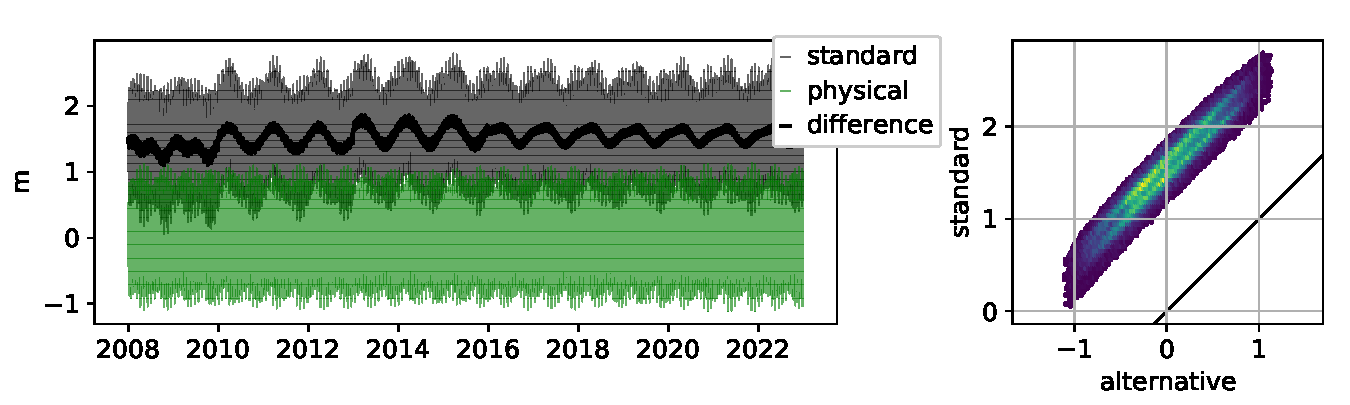
\includegraphics[width=\figwidthFull]{figures/plots/piecewiseTide_62430.png}
        \caption{Contrast between concatenated official predictions and a hindcast based on ``weather-free'' latest tidal parameters at \Dname{}.  Note the intentional discontinuities in official predictions associated with annual updates and growing input record length.   (....TBC may overlay ACCESS-S data too) }
    \label{fig:tideOverlay}
\end{figure}   

%------------------------------------------------
\section{Proposed split of content types for an automated tidal data service}
\label{Sec:proposed}

Novelty is the very idea of asking the conventional service to move away from a single 'tide'.
AN incremental shift can be made without significant technological change - but will enable future and ongoing improvements free from the untenable conceptual constraints. 

Adding complexity to operational systems is generally bad and a good data service just ``does what it says on the box''.  But considering the diverse uses for synthesised tidal signals, the following are considered to be requirements : 
\begin{itemize}
    \item deliver data at arbitrary time stamps
    \item isolate users from details of backend software 
    \item distinguish a physical tide estimate from official standard predictions
    \item allow for differentiation between forecast, hindcast and analysis
    \item explicate historical reference datum and MSL change components
    \item provide rankable quality measures
\end{itemize}

With these motivations in mind, the following ``flavours'' are put forwards as an incremental step towards ensuring conventional tide services can compliment modern uses.   Emphasis is placed on conveying the need for \textit{any} signal split rather than exact wording and finer details.
Further justification and illustration of the significance of these distinctions is addressed in the subsequent sections.

\begin{table}[H]\centering
    \begin{tabular}{ |c|c|c|c|c| }
    \hline
    name    & 
        default reference  & 
        issue date         & 
        valid time limits  \\
    \hline
    official tide prediction [\ref{Sec:flavour1}] & 
        chart datum & annual & 
        concatenated bounds\\
    \hline
    physical tide prediction [\ref{Sec:flavour2}]& 
        MSL       & 
        arbitrary & 
        no limit \\
    \hline
    physical tide analyses [\ref{Sec:flavour3}]& 
        MSL       & 
        arbitrary & 
        within observation range \\
    \hline
    \end{tabular}
    \caption{summary of proposed data types}
    \label{tab:typesSummary}
\end{table}

NOTE - contrast to the importance of observations and repoisitories like Gelsa and UH.

NOTE - different to just bandlimited signals.  Should allow for long period content in the weather-free... cf Flinchem.


Plenty of room for refinement, but regardless we have a simple representation error problem where primarily weather-driven variations are projected onto tidal analysis.
 
%------------------------
\subsection{Official reference prediction timeseries}
\label{Sec:flavour1}
Official predictions have a special legal status both directly for  navigation purposes and indirectly for some other applications.   
For instance the Australian Navigation Act \cite{AusNavAct2012} details a requirement for vessels to carry nautical publications, and specifically tide tables, from the official charting authority.  Charted depths are defined relative to a datum generally aligned with the Lowest Astronomical Tide value derived from synthesised official tidal timeseries over a fixed period \cite{PCTMSL-sp9}.
Any API delivery of official tides must be consistent with these regulatory requirements.  Moreover, inclusion of this prediction type is obvious and should form the core of any national service.


Official predictions are forecasts that aim to represent the total still-water level under average conditions. ``\textit{As predictions are given for average meteorological conditions it follows that when conditions are not average the actual tides may differ from those predicted.}''\citep{austides}


Official predictions are traditionally issued annually for a 1 year period.  
Discontinuities are possible between annual predictions. Most overtly if the prediction datum is changed,  but also due to the annual revision of prediction parameters.
Providing access to \textit{historical} official predictions therefore requires an API to handle forecast-valid dates.  Note that this requirement rules out the possibility of using a single set of contemporary tidal parameters to synthesise a hindcast for any arbitrary historical period on-the-fly.
Figure \ref{fig:tideOverlay} provides examples to illustrate this distinction. 

%------------------------
\subsection{Physical `weather-free' tide forecast timeseries}   
\label{Sec:flavour2}
There are valid use-cases for tide predictions that do not align with the regulatory aims of traditional forecasts; both with respect to the ``official'' status of the annual promulgation and also regarding the component of total sea level that is being targeted.

It is asserted that many such cases require tide predictions to be the best available estimate of the tidally-driven component of total sea level.   Rather than a prediction of still water level under average conditions this a prediction of a physical component \textit{regardless} of meteorological conditions.  
There is no reason to restrict the revision of these un-official predictions to an annual update cycle.

Combination of harmonic tide predictions with dynamic model forecasts is one use-case \citep{Taylor:2017coa} that is discussed further in Section \ref{Sec:DoubleCount}.
Any data-driven methodology that involves the filtering of real-time tide gauge observations in order to ingest or assimilate non-tidal residuals would also be better served  
eg \cite{10.3389/fmars.2019.00437}.
Furthermore, residuals derived using such a ``weather-free'' tide prediction prima facie share a more consistent representational target as the sea level anomaly (SLA) data derived from satellite altimetry - discussed further in Section \ref{Sec:OfficialGlobal}.


This flavour of prediction is simply what physical oceanography has largely thought of as `tides' for decades \cite{Munk:1966ts} despite the fact that response method techniques ``\textit{...have never been adopted for ordinary tide-table production [and] remain essentially a research tool for specialists}''\citep[p.198]{Cartwright:2000tt}.
The contemporary operational context has however increasingly brought conventional tide-tables and physical oceanography into the same space and the micro-service service architecture should support this without contradiction. 
      
%------------------------
\subsection{Behind-real-time quality tide analysis timeseries}  
\label{Sec:flavour3}
 
NOTE - allows for accounting for the modulation and/or temporary evolution.    No reason to remain tied to harmonic or prediction methods.    Eg open to application of wavelets or whatever.


 
The behind-real-time partner to the weather-free prediction (\ref{Sec:flavour2}) is the weather-free analysis.   The distinction being analogous to that between a weather model forecast and analysis or the IGDR and GDRs of satellite data \cite{Picot:2003tp}.   
The dual meaning of 'analysis' for both the tidal process and the timeseries here is unfortunate but unavoidable and hopefully clarified by context. 

This flavour would serve as a de-tiding filter for historical observations, as an evaluation target for behind-real-time regional tide modelling  \cite{10.5194/os-2020-107} and potentially as an input to geophysical re-analysis such as \cite{10.1029/2017jc013685}.

%------------------------
\subsection{Spatial metadata and levels}
Metadata regarding the location, identity and especially relative elevation of tidal timeseries is fundamental to a useful API.
Vertical datum transformation and unification is an active area of development is Australia (\cite{Keysers:we}\cite{Filmer:2018cu}\cite{AVWS2021}).   The details are beyond the scope of the present discussion, but the relationship between prediction datum and the ellipsoidal references employed in modern positioning is highlighted as carrying special relevance.

%------------------------
\subsection{Rankable quality measures}

Whilst high quality, continuous long records of sea level observation are ideal for tidal methods, in practice this is only available for a relatively small network of tide gauges.   

The schematic in Figure \ref{fig:tidePractice} conveys the attractive ability of conventional tidal practice to produce uniform outputs from a very heterogeneous set of inputs.
Uniformity of format is not the same as uniformity of quality, but without appropriate supporting information users of tidal data would be left to treat all predictions as equal.  

Australian systems currently have effectively only two quality categories: `primary' and `secondary' \cite{austides} that are sometimes also designated `standard' and `subordinate'  \cite{PCTMSL-sp9}.   
It is also common to see unofficial tide predictions clearly marked as ``not for navigation'' for various reasons.


This binary classification is not sufficient for many applications and it is asserted that the major deficiency is the lack of ability to rank by quality.   There are several dimensions by which synthesized tidal timeseries could be assigned rankable quality measures.    
The analysed observational record length is at least one practical candidate and specifically highlighted by \cite{MHL2156}. But the bespoke analysis process, for instance involving inference or moved stations \cite{godin:1972}), can render record length more ambiguous than at first may be apparent.    
Related to record length is the candidate measure of extrapolation time, to quantify the time period prior-to or after the analysed observational record.     
A quality measure that reflects skill relative to an independent period of water level observations could also provide useful guidance to users of the data.    In contrast, any measure derived directly from the tidal analysis itself (inversion) would require care to avoid over-fitting and circular reference \cite{Thompson2019}. 


The absence of rankable quality measures left Griffin et al \citep{10.5194/os-2020-107} to rely on a needlessly empirical blacklisting procedure to reject tidal analysis sites from a simulation evaluation on the basis of being of grossly poor quality. Such information should readily accompany machine-readable tidal data.


%------------------------------------------------
\section{Discussion}
\label{Sec:Discussion}

Why incremental?

Long history of proposed new methods and details for tides.
Conventional harmonic methods are so well embedded and provide unique forecast value that is sure to persist for some time to come.

Motivation to provide automated (eg web API) data delivery presents a good chance to review and incrementally nudge the service in a helpful direction.

Perhaps analogous to Devin and Zaron Jay etc nudging progress not by discarding the traditions of tidal analysis, but subtly adapting to primfacie contrasting ideas: 'nonstationary tides' or 'tidal variablity' etvc.


Worth the trouble?
Significance of harmonics ...only 10s  of centimeters.   But scales like this are worth some attention when consider the increased frequency of nuisance flooding etc
And anything that helps progress the clarity of refrence datums in the coastal zone would be most welcome ...


Basic service design can set the stage for
Enable expansion of down-stream uses and avoid needless representational confusion.
whilst ...
Enable ongoing backend improvements without need to draw too many compromises for different use-cases.

%%%%%%%%%%%%%%%%%%%%%%%%%%%%%%%%%%%%%%%%%%
%\end{paracol}
%\input{post}
%\reftitle{References}

% Please provide either the correct journal abbreviation (e.g. according to the “List of Title Word Abbreviations” http://www.issn.org/services/online-services/access-to-the-ltwa/) or the full name of the journal.
% Citations and References in Supplementary files are permitted provided that they also appear in the reference list here. 

%=====================================
% References, variant A: external bibliography
%=====================================
%\externalbibliography{yes}
%\bibliography{your_external_BibTeX_file}
%\bibliography{references}
